\documentclass{IEEEtran}
\usepackage{bm}
\usepackage{amsmath}
\usepackage{graphicx}
\usepackage{amsmath}
\DeclareMathOperator*{\argmax}{arg\,max}
\DeclareMathOperator*{\argmin}{arg\,min}
\renewcommand{\IEEEQED}{\IEEEQEDclosed}
\title{Optimal Fishing Strategy Based on Scientific Concept of Development}
\author{
    Weitong~ZHANG, Yiwen~LU, Zifeng~KANG*
    \thanks{Weitong~ZHANG 2015011493 Email: zwt15@mails.tsinghua.edu.cn}
    \thanks{Yiwen~McF.~LU 2015011443 Email: ylu.thu15@gmail.com}
    \thanks{Zifeng~KANG 2015011??? Email: sklearn@python.org}
}
\begin{document}
\maketitle

\begin{abstract}
    The SOD incorporates scientific socialism, sustainable development, social welfare, a humanistic society, increased democracy, and, ultimately, the creation of a Socialist Harmonious Society. According to official statements by the CPC, the concept integrates "Marxism with the reality of contemporary China and with the underlying features of our times, and it fully embodies the Marxist worldview on and methodology for development."
\end{abstract}

\section{Introduction}
\section{Basic Assumptions}
\section{Model on Sustainable Harvesting} \label{model1}

Owing to the annual death ratio is 0.8, we assume that the number of fish $x$ obeys the distribution eq. \ref{eq1}

\begin{equation}
    \label{eq1}
    x = x_0 \exp(-\lambda t)
\end{equation}

while the unit of $t$ is year, we get $\lambda = \ln 5, \frac{\mathrm dx}{\mathrm dt} = -\lambda x$

Setting the fishing intensity of 4-aged fish to be $k$, we can get the one of 3-aged fish is $0.42k$, while the number of the four group of fish could be described as a 4-d vector $\bm x$ .

\subsection{Model on the first eight years}

We can use the differential equation eq. \ref{eq2} to describe the trend of the number of fish in each group

\begin{align}
    \label{eq2}
    -\frac{\mathrm d \bm x}{\mathrm d t} &= k \mathbf C \bm x + \lambda \bm x \\
    \mathbf C &= \begin{pmatrix}0&0&0&0\\0&0&0&0\\0&0&0.42&0\\0&0&0&1\end{pmatrix}
\end{align}
\subsection{Model on the last four month}
Set the number of eggs is $y$, and for each fish, we set the rate of spawning is $\mu$, i.e. $\frac {\mathrm d y_i}{\mathrm d t} = \mu$, where $y_i$ is the eggs spawned by a certain fish $i$. Then we get the following differential equation eq. \ref{eq3}

\begin{align}
    \label{eq3}
    \frac {\mathrm d y}{\mathrm d t} &= \mu \mathbf D \bm x\\
    -\frac{\mathrm d \bm x}{\mathrm d t} &=\lambda \bm x\\
    \mathbf D &= \begin{pmatrix} 0 & 0 & 1.109\times10^5/2&1.109\times10^5\end{pmatrix}
\end{align}

From the average spawning rate, we can get that $\mu = 3$.

\subsection{Model on the changes of the next year}

After a year, some eggs spawned in the first year would be the 1-aged fish, according to the survival ratio. Therefore, we can get the following transform function eq. \ref{eq4}

\begin{align}
    \label{eq4}
    y &= 0\\
    \bm x &= \mathbf T \bm x +\begin{pmatrix} f(y)&0&0&0\end{pmatrix}^{\mathrm T}\\
    f(y) &= \frac{1.22\times 10 ^{11}y}{1.22\times 10 ^{11} + y}\\
    \mathbf T &= \begin{pmatrix} 0 & 0 & 0 & 0 \\ 1& 0 & 0 & 0 \\ 0 & 1 & 0 & 0 \\0 & 0 & 1 & 1 \end{pmatrix}
\end{align}

\subsection{Solve the function}

Now We can conclude all of the function above to solve the equation \ref{eq5} of $\bm x$: $\bm x' = \bm x$ based on $k$, where $\bm x'$ is the number of fish next year:  

\begin{equation}
    \label{eq5}
    \bm x_0 = \mathbf T \exp(-\frac{\mathbf A_2 + 2 \mathbf A_1}{3})\bm x_0 +\begin{pmatrix} f(\mathbf B \exp(-\frac{2\mathbf A_1}{3})\bm x_0)&0&0&0\end{pmatrix}^{\mathrm T}
\end{equation}
\begin{align}
    \mathbf A_1 &= k\mathbf C + \lambda \mathbf I\\
    \mathbf A_2 &= \lambda \mathbf I\\
    \mathbf B &= (\mu \mathbf D A_2^{-1}(\mathbf I - \exp(-\mathbf A_2/3)))
\end{align}

Therefore, we can get the relationship between $\bm x$ and $k$ numerically.
\subsection{Relation bewteen Harvest and Fishing Intensity}
The total of harvest $z$ could be described as the following function eq. \ref{eq6}

\begin{align}
    \label{eq6}
    \frac {\mathrm dz}{\mathrm dt} &= k\mathbf C \vec x\\
    z &= k\mathbf C\int_0^{2/3}\exp(-\mathbf A_1t)\mathrm dt\bm x_0 \\ 
    &= k\mathbf C  A_1^{-1} (1-\exp(-2\mathbf A_1/3))\bm x_0
\end{align}

where $\bm x_0$ would be the initial number of fish.

\subsection{Numerical result and Optimize $k$ for maximizing $z$}

By numerical method, we can get the final relationship between the $k$ and the total havest $z$, which could be plotted as ...

%%%%%%%%%%%%%%%%%%%%%%%%%%%%%%%%%%%%%%%%%
%
%         RESULT FOR PART 1
%
%%%%%%%%%%%%%%%%%%%%%%%%%%%%%%%%%%%%%%%%%
\section{Model on five successive fishing}

According to the 
\section{Result}

\subsection{Solution to the first problem}

Applying the model described in Part \ref{model1}, under the constraint of sustainable harvesting, the annual harvest $z$ can be plotted in terms of the fishing intensity of 4-aged fish $k$, as is shown in Figure \ref{plot1}. Note that $z$ is meaningful if and only if $z>0$, and thus the feasible region of $k$ is automatically determined.

\begin{figure}[h]
	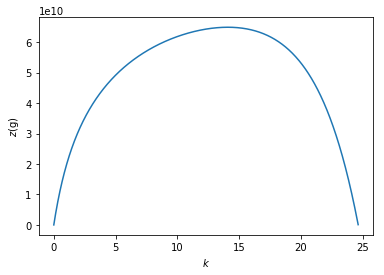
\includegraphics[width=\columnwidth]{plot1}
	\caption{The relationship between annual harvest $z$ and fishing intensity $k$\label{plot1}}
\end{figure}

The relationship between $z$ and $k$ is not monotonous, which agrees with our intuition: when $k$ is too small, the fishing intensity is too small to exploit the resources; when $k$ is too large, the number of fishes in the steady state is decreased, affecting the harvest. By performing a linear search on $k$, the optimal fishing strategy can be determined:

$$\begin{cases}\argmax\limits_k z(k) \approx 13.41\\\max\limits_k z(k) \approx 6.39\times 10^{10} \end{cases}$$

\subsection{Solution to the second problem}



\section{Conclusion}
\end{document}